\documentclass[11pt,a4paper,final]{article}
\usepackage[utf8]{inputenc}
\usepackage{amsmath}
\usepackage{amsfonts}
\usepackage{amssymb}
\usepackage{graphicx}
\usepackage{hyperref}
\usepackage[left=2cm,right=2cm,top=2cm,bottom=2cm]{geometry}
\author{Franziska Metge}
\title{Finding your next vacation spot} 
\begin{document}
\maketitle
\section{Introduction}
\subsection*{Problem}
We live in a world of travelers but we also live in a world of individuals with divers interests. It would be preposterous to assume that everybody enjoys exactly the same cities. Some people might enjoy cities with a good night life, while others want to travel to cities with a diverse cultural landscape. 

\subsection*{Background}
Traveling greatly promotes personal growth, hence I try to travel somewhere new every year. By now I have traveled to most European capitals and other major cities. Each year it becomes harder and harder to pick a city and I have also encountered cities that I did not enjoy visiting. One major reason was that they were too crowded with tourists (I understand irony of the problem). For my next travel destination I would like to select a less popular city, while ensuring that the city is similar to what I have enjoyed before. 

\subsection*{Solution}
Therefore I will develop a program which is able to find cities a user might find enjoyable based on an input city and venue landscape. I will implement the code in an Ipython notebook and will make use of the python libraries introduced in the Machine Learning Course such as \texttt{numpy}, \texttt{pandas}, and \texttt{sklearn}. The program will return as many similar cities as desired. Besides a table listing the similar cities, the program will return a heat-map visualizing the similarity of these cities by venue occurrence. A scatter-plot using the cities coordinates will also be returned. This material will enable the user to confidently select their next travel destination.

\subsection*{Target audience}
My idea is intended to be used by people who are looking for a new travel destination spanning further than all the known classics like Paris or New York. A user will be able to make the most of the program if they had already traveled to a considerable amount of cities and know what they appreciated. 

\section{Data}
I will use the population data made publicly available by the United Nations (\href{https://unstats.un.org/unsd/demographic-social/products/dyb/documents/DYB2018/table08.xls}{Demographic Yearbook – 2018}\footnote{\url{https://unstats.un.org/unsd/demographic-social/products/dyb/dyb_2018/}}). I will use \texttt{numpy} and \texttt{pandas} libraries to clean the data. An example of this data is given in table \ref{tab:pop_data}.

\begin{table}[h!]
\centering
\scalebox{0.6}{
\begin{tabular}{|l|r|c|}
\hline
\textbf{City} & \textbf{Population Size} & \textbf{Country} \\\hline
Adrar & 200834.0 & Algeria \\
Ain Defla & 450280.0 & Algeria \\
Ain Temouchent & 299341.0 & Algeria \\
ALGIERS (EL DJAZAIR) & 2712944.0 & Algeria \\
Annaba & 442230.0 & Algeria \\
Batna & 768444.0 & Algeria \\
Béchar & 236213.0 & Algeria \\
Bejaïa & 559981.0 & Algeria \\
Beskra (Biskra) & 563245.0 & Algeria \\\hline
\end{tabular}}\caption{Cleaned population data}\label{tab:pop_data}
\end{table}

Secondly, I will use the \texttt{geopy} library to acquire the coordinates for all cities. I will separate cities into different classes/groups based on their population size, i.e. $ < 0.5\text{ Mio}, 0.5-1\text{ Mio}, 1-5\text{ Mio}, 5-10\text{ Mio}, 10-20\text{ Mio}, \text{and} >20\text{ Mio}$ (see Table: \ref{tab:pop_coordinates}).\\

\begin{table}[h!]
\centering
\scalebox{0.6}{
\begin{tabular}{|l|r|c|r|r|c|}
\hline
\textbf{City} & \textbf{Population Size} & \textbf{Country} & \textbf{Latitude} & \textbf{Longitude} & \textbf{population\_bin} \\\hline
Adrar & 200834.0 & Algeria & 27.9458867 & -0.1992938330258469 & 1 \\
Ain Defla & 450280.0 & Algeria & 36.15868425 & 2.084281730358365 & 1 \\
Ain Temouchent & 299341.0 & Algeria & 35.26665705 & -1.149927622407504 & 1 \\
ALGIERS (EL DJAZAIR) & 2712944.0 & Algeria & 36.7753606 & 3.0601882 & 3 \\
Annaba & 442230.0 & Algeria & 36.8982165 & 7.7549272 & 1 \\
Batna & 768444.0 & Algeria & 35.3384291 & 5.731545299000572 & 2 \\
Béchar & 236213.0 & Algeria & 31.62298095 & -1.914198993519679 & 1 \\
Bejaïa & 559981.0 & Algeria & 36.7511783 & 5.0643687 & 2 \\
Beskra (Biskra) & 563245.0 & Algeria & 34.7845635 & 5.812435334419206 & 2 \\\hline
\end{tabular}}\caption{Cities with coordinates}\label{tab:pop_coordinates}
\end{table}

I will use the \texttt{Foursquare API} to look for all venues within a 5km radius of the city's center (see Table: \ref{tab:venues}). 

\begin{table}[h!]
\centering
\scalebox{0.6}{
\begin{tabular}{|l|r|r|l|r|r|l|}
\hline
\textbf{City} & \textbf{City Latitude} & \textbf{City Longitude} & \textbf{Venue} & \textbf{Venue Latitude} & \textbf{Venue Longitude} & \textbf{Venue Category} \\\hline
Adrar & 27.9458867 & -0.1992938330258469 &  &  &  &  \\
Ain Defla & 36.15868425 & 2.084281730358365 &  &  &  &  \\
Ain Temouchent & 35.26665705 & -1.149927622407504 & Fast food Le Loft & 35.2949989986954 & -1.137600108318426 & Fast Food Restaurant \\
ALGIERS (EL DJAZAIR) & 36.7753606 & 3.0601882 & Restaurant Le Thyrolien & 36.77518773893406 & 3.058731268449381 & BBQ Joint \\
ALGIERS (EL DJAZAIR) & 36.7753606 & 3.0601882 & CARACOYA & 36.76667223648845 & 3.053610267518587 & French Restaurant \\
ALGIERS (EL DJAZAIR) & 36.7753606 & 3.0601882 & "TNA ""Théâtre National d'Alger""" & 36.78097827704275 & 3.060508018126319 & Theater \\
ALGIERS (EL DJAZAIR) & 36.7753606 & 3.0601882 & Didouche Mourad & 36.76557038107158 & 3.051074029384855 & Plaza \\
ALGIERS (EL DJAZAIR) & 36.7753606 & 3.0601882 & Tantonville & 36.780824 & 3.06031 & Café \\
ALGIERS (EL DJAZAIR) & 36.7753606 & 3.0601882 & Musée d'Art Moderne Algérie & 36.77720262790217 & 3.058272841808561 & Art Museum \\\hline
\end{tabular}}\caption{Foursquare results}\label{tab:venues}
\end{table}


The data will be stored in a table with one row per city containing the cities name, country, coordinates, population size, population size category, number of venues from different categories in one-hot encoding (see Table \ref{tab:one_hot} ).\\

\begin{table}[h!]
\centering
\scalebox{0.6}{
\begin{tabular}{|l|r|l|r|r|c|c|c|c|c|c|}
\hline
\textbf{City} & \textbf{Population Size} & \textbf{Country} & \textbf{Latitude} & \textbf{Longitude} & \textbf{population\_bin} & \textbf{ATM}& \textbf{...} & \textbf{Fast Food Restaurant} & \textbf{... }& \textbf{Zoo Exhibit} \\\hline
Ain Temouchent & 299341.0 & Algeria & 35.26665705 & -1.149927622407504 & 1 & 0 & & 1 & & 0 \\
ALGIERS (EL DJAZAIR) & 2712944.0 & Algeria & 36.7753606 & 3.0601882 & 3 & 0 & & 0 & & 0 \\
Annaba & 442230.0 & Algeria & 36.8982165 & 7.7549272 & 1 & 0 & & 0 & & 0 \\
Bejaïa & 559981.0 & Algeria & 36.7511783 & 5.0643687 & 2 & 0 & & 0 & & 0 \\
Bordj Bou Arreridj & 422986.0 & Algeria & 36.095506 & 4.661100173631754 & 1 & 0 & ... & 0 & ... & 0 \\
El Bayadh & 192958.0 & Algeria & 33.63785225 & 1.012203911250456 & 1 & 0 & & 0 & & 0 \\
Guelma & 363716.0 & Algeria & 36.3491635 & 7.409498952760461 & 1 & 0 & & 0 & & 0 \\
Jijel & 391096.0 & Algeria & 36.8167305 & 5.771494 & 1 & 0 & & 0 & & 0 \\
Laghouat & 371204.0 & Algeria & 33.8063518 & 2.8808616 & 1 & 0 & & 0 & & 0 \\\hline
\end{tabular}}\caption{One-hot endcoding of input data}\label{tab:one_hot}
\end{table}

Table \ref{tab:one_hot} will be the input table used for my program. Based on the columns \textbf{ATM} to \textbf{Zoo Exhibit} the function will calculate a similarity score between all cities using the function \texttt{pdist} from the package \texttt{sklearn}.



\section{Methods}
\subsection{Exploratory data analysis}
In order to get a general impression of the data I will first do a principal component, a t-Distributed Stochastic Neighbor Embedding, histograms and a scatter plot comparing number of venues against number or different venues per city.
\subsubsection*{PCA}
A principal component analysis (PCA) is a dimensionality reduction to visualize high dimensional data in a low dimensional space while keeping the relation between points (i.e. points closer in high dimensional space will be closer in low dimensional space than more distant points). Before calculating the components I will first scale the data using \texttt{sklearn.preprocessing.StandardScaler} to make sure all features have equal weights when calculating the components. I will use the python function \texttt{decomposition.PCA} from the package \texttt{sklean} to calculate principal components. 
\subsubsection*{t-SNE}
A t-Distributed Stochastic Neighbor Embedding (t-SNE) is a different dimensionality reduction method. I will use the function \texttt{TSNE} from \texttt{sklearn.manifold} with the default parameters to calculate the new embedding.
\subsubsection*{Histogram}
I will use the \texttt{distplot} function from \texttt{seaborn} to visualize an overview of first how many venues there are of each category and second how many venues there are in each city.
\subsubsection*{Correlation}
Lastly, I will inspect the relationship between the number of different categories per city against the total number of venues per city using the \texttt{seaborn} function \texttt{regplot}. I will also calculate the Pearson correlation coefficient using the \texttt{scipy.stats} function \texttt{pearsonr}.

\subsection{Implemented functions}
To execute my idea I implemented two functions. In the following section I will explain how these functions work in detail.

\subsubsection*{\texttt{find\_next\_vacation}}
The first function \texttt{find\_next\_vacation} returns a list of cities that are similar to the given input city. The function depends on the city-venue data in an one-hot encoding like structure (see Table \ref{tab:one_hot}), an input city name, number of similar cities to return, and the similarity measure to be used. \\  
First, a distance matrix is calculated using the \texttt{pdist} from the \texttt{scipy.spatial.distance} package. Secondly, based on the similarity score, the \texttt{k} most similar cities to the input cities are selected and the city-venue table is sub-setted to only these cities, including the input city. All venue categories not present in the input city are removed. Columns are then sorted from highest to lowest occurrence in the input city. Rows are sorted from most similar to the the input city to least similar to the input city. \\  
This data is returned to the user. Furthermore, the venue occurrence by city and category is visualized in a heat map. The similar cities are visualized in a scatter plot by using x='Longitude' and y='Latitude', mapping the population size as dot size and the similarity score as color. This will give the user a visual overview allowing to make a quick selection of future travel destinations.

\subsubsection*{\texttt{get\_information\_on\_next\_vacation}}
The second function \texttt{get\_informatin\_on\_next\_vacation} can be used to obtain venues that can be found in the selected city. The function depends on the output table generated by \texttt{find\_next\_vacation}, a selected city and the number of venues to return. \\
The function uses the \texttt{Foursquare API} to find venues of the given city based on the coordinates obtained from the input table, i.e. such that the user only needs to select a city. The function returns the found venues in the same table format as examplarized in Table \ref{tab:venues}.

\subsection{Applying implemented functions}
I will apply the aforementioned functions to five input examples. The following code demonstrates how the functions are executed.

\begin{verbatim}
# first function:
future_vacation_destination_Berlin = find_next_vacation('BERLIN', 
                                     population_venue_data, 10, 
                                     'euclidean')

# second function:
future_vacation_destination_info = get_information_on_next_vacation('s-Gravenhage',
                                   future_vacation_destination_Berlin, 20)
\end{verbatim}


\section{Results}
\subsection{Exploratory data analysis}
Figure \ref{fig:pca_tsne} shows the two different dimensionality reduction embedding of the data. Both pictures show a big cloud of data points and a smaller group of data points separated from the big cloud. There are no clear trends in the data with respect to population size. 

\begin{figure}[h!]
\begin{center}
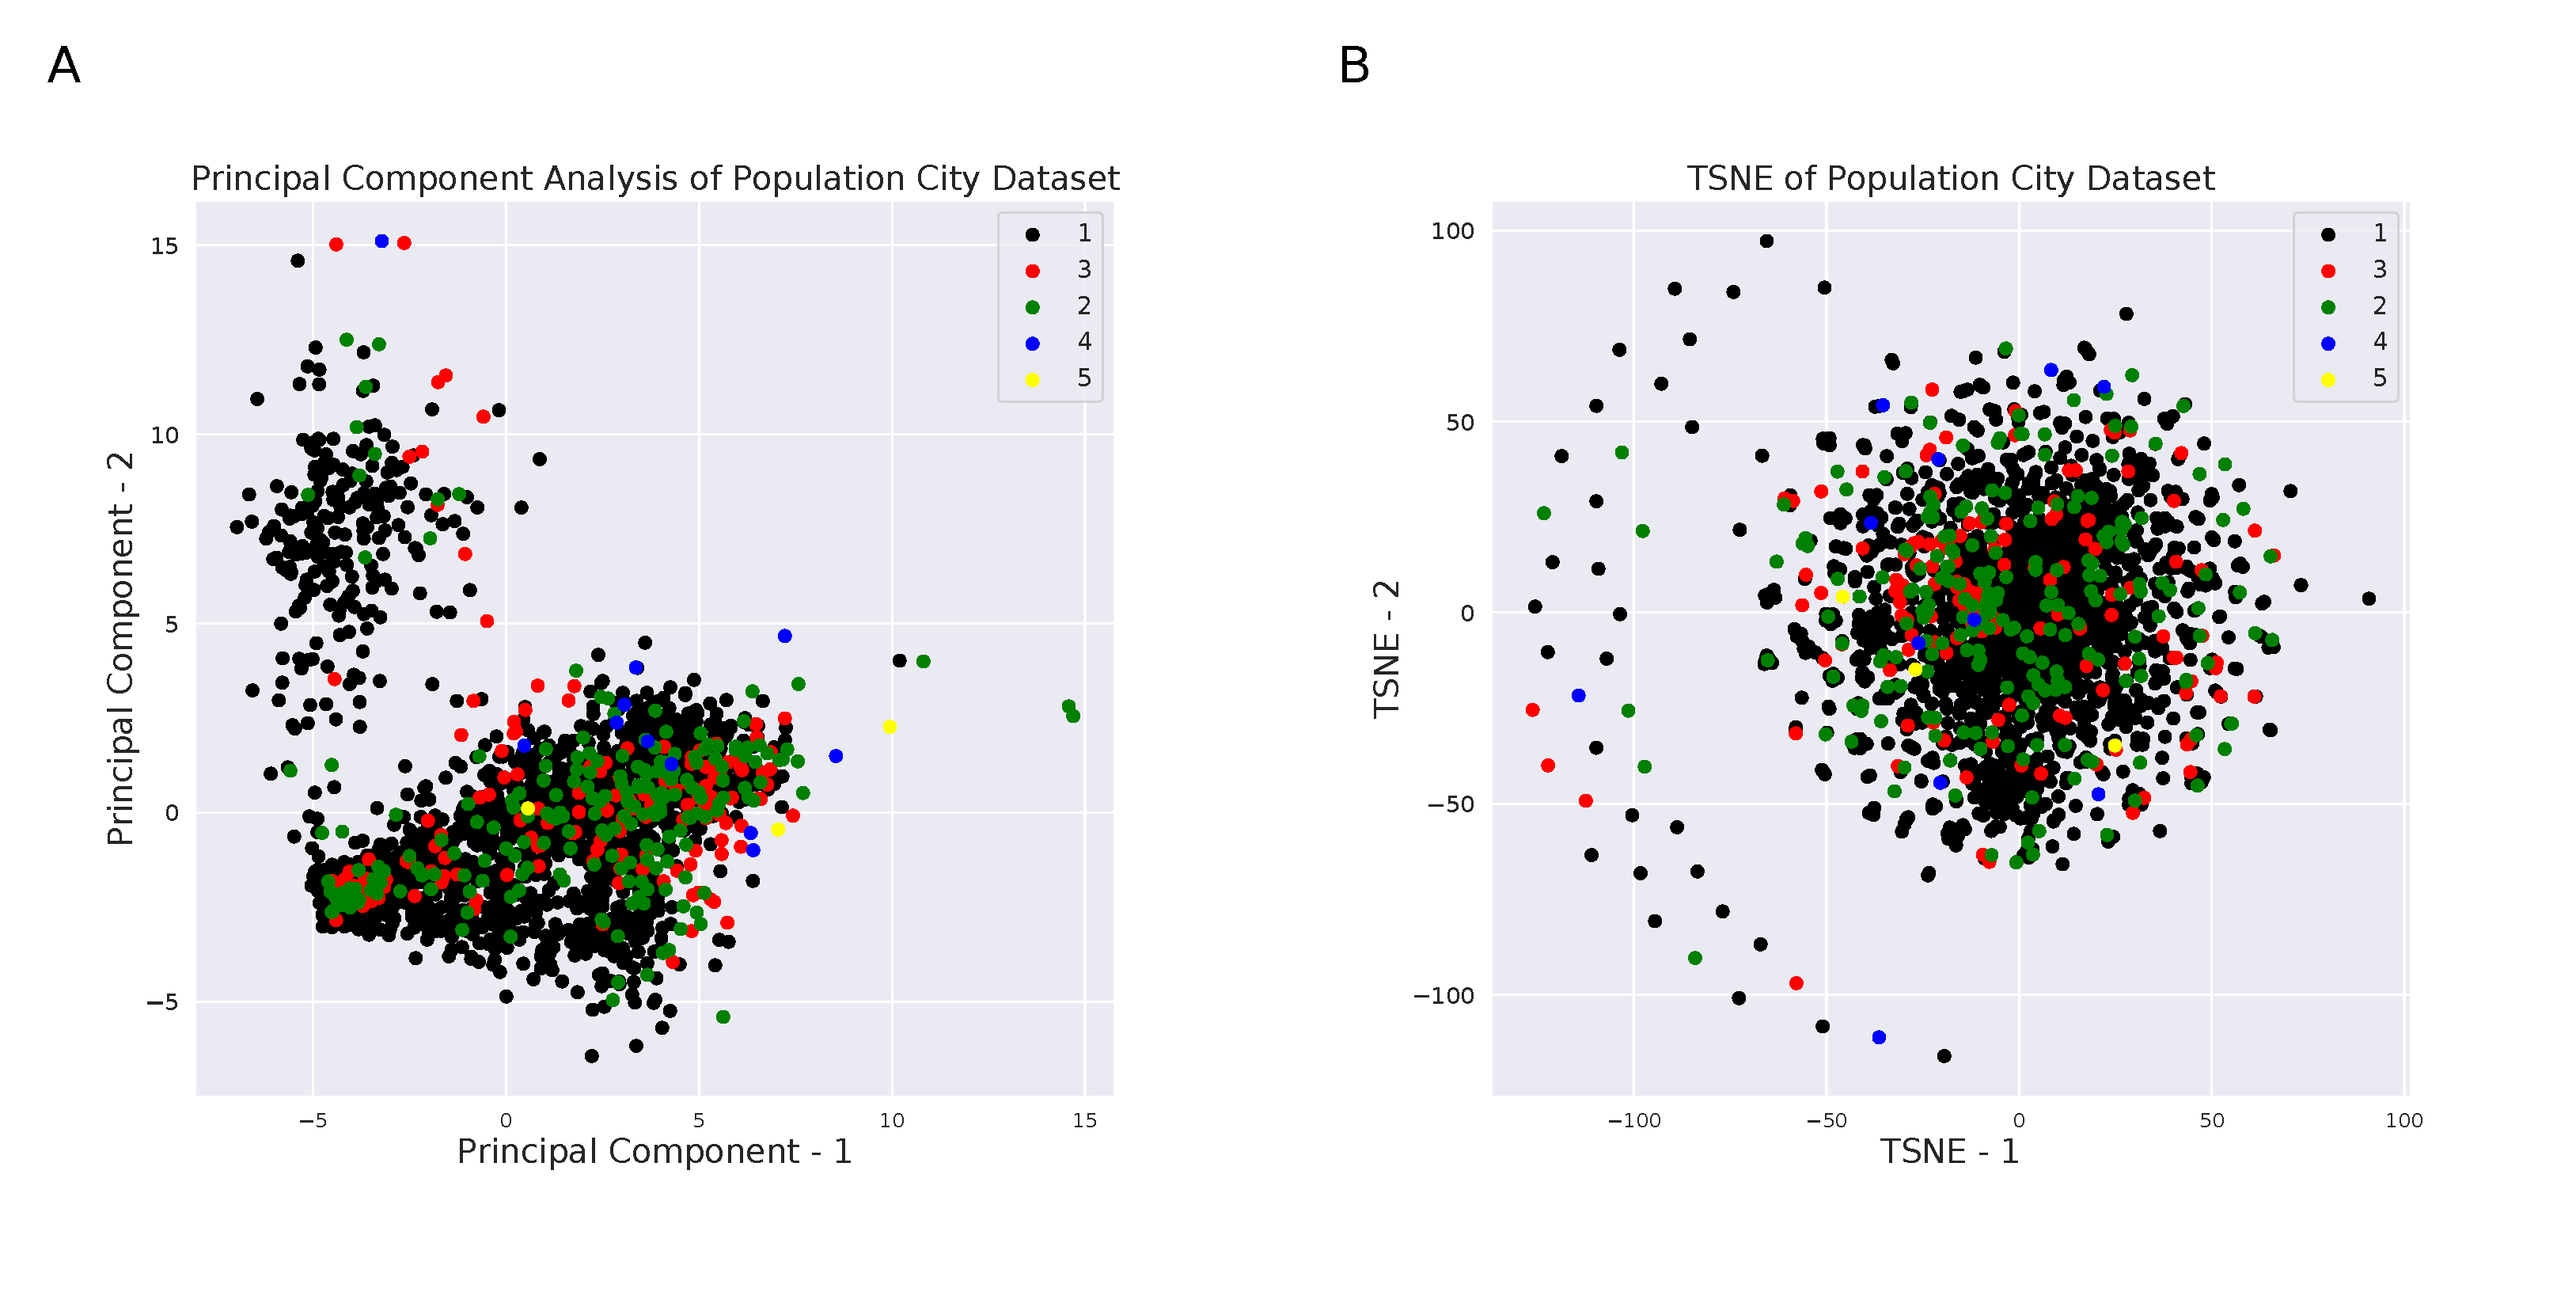
\includegraphics[width = 1\textwidth]{figures/fig1.pdf} 
\caption{A) Principal component analysis. This figure shows an embedding of the data onto the first and second component. The second component separates a group of cities from the denser cloud. B) t-SNE projection. This figure shows an embedding of the data onto the first and second axis. This embedding also shows a separation of a dense cloud and outliers.}\label{fig:pca_tsne}
\end{center}
\end{figure}

Figure \ref{fig:histograms} shows the distribution of venues across categories, across cities, and the relation ship of number of venues (venue abundance) and absolute number of different categories (venue diversity) over all cities. \\
Figure \ref{fig:histograms} A shows that a large majority of categories only occur between 1 and 250 times. A few outliers are as abundant as 7000 times such as hotels, cafes, and coffee shops. \\ 
Figure \ref{fig:histograms} B shows a bimodal distribution clearly highlighting the limit of 100 venues per city, potentially underestimating the true venue landscape of many cities.\\
Figure \ref{fig:histograms} C correlates the number of venues per city with the number of different venue categories that can be found in a city. This high correlation ($R_{pearson} = 0.95$) indicates that cities with more venues are also more diverse and do not just offer more of the same venue type. However, it becomes evident that summarizing the one-hot encoded city-venue table by city alone instead of city and country leads to a miss-assignment of venues to cities causing some cities to have more than 100 venues. As explained before, this should not be possible.

\begin{figure}[h!]
\begin{center}
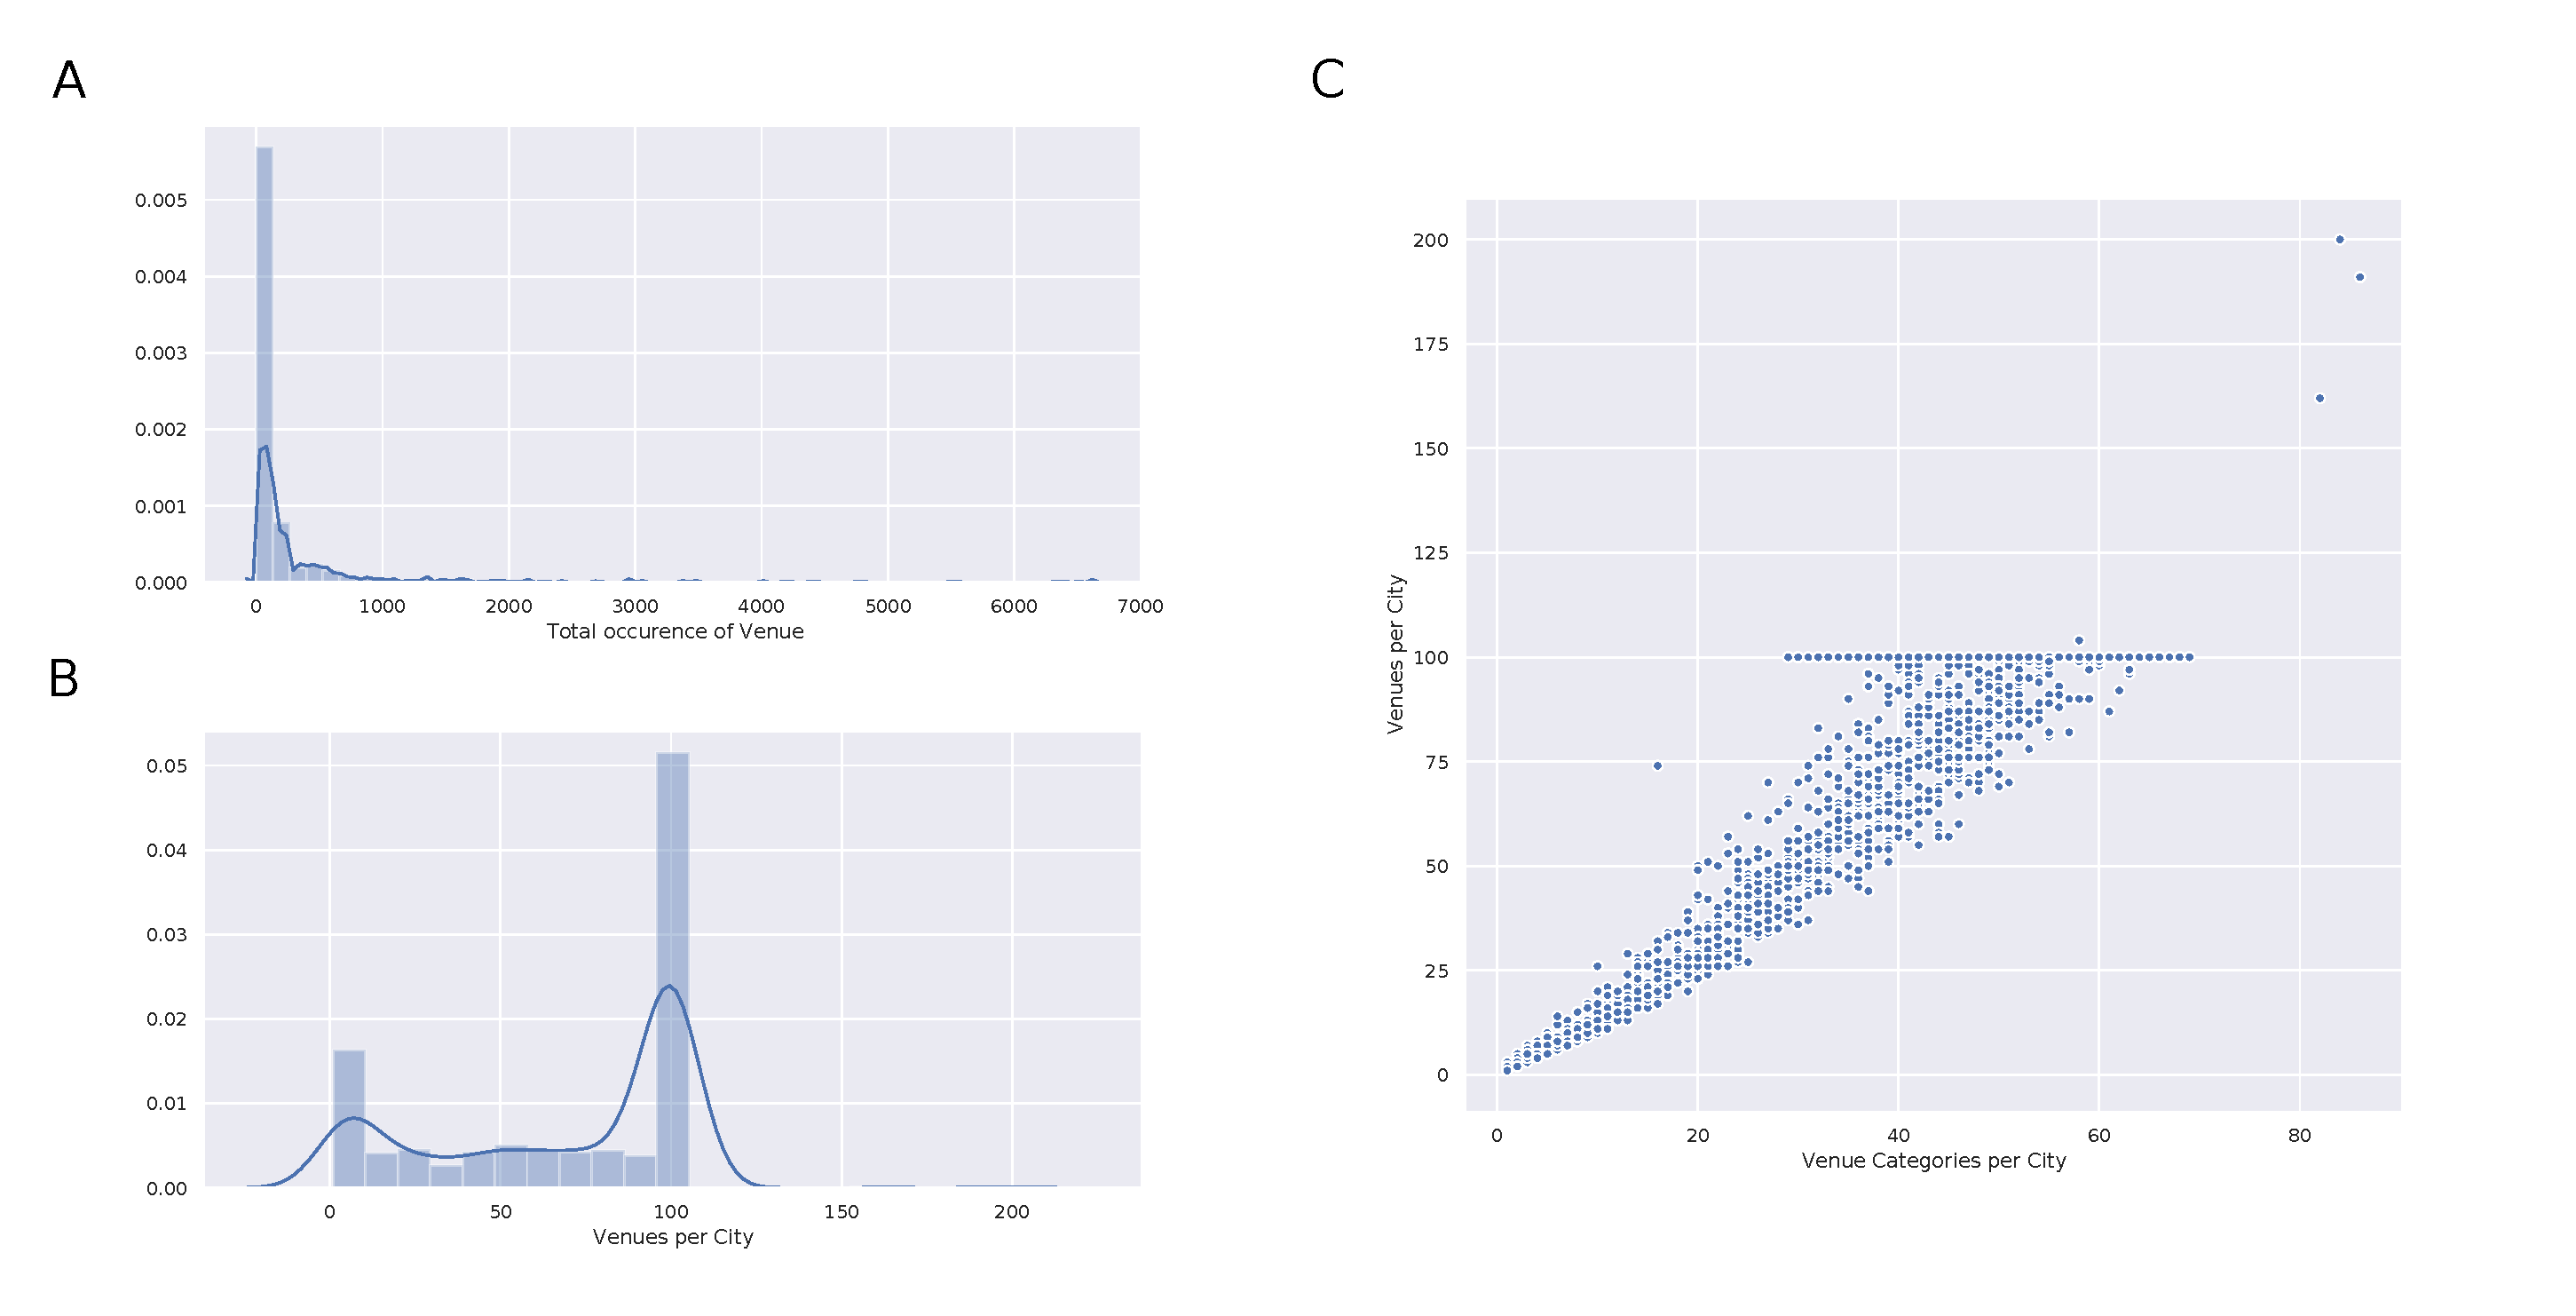
\includegraphics[width = 1\textwidth]{figures/fig2.pdf} 
\caption{A) Distribution of how often each type of venue occurs, i.e. there are 6593 coffee shops in the data set. B) Distribution of number of venues per city C) Correlation of venues per city and categories per city highlighting the increasing diversity.}\label{fig:histograms}
\end{center}
\end{figure}

\subsection{Applying the functions}

I applied my newly developed function using five different input cities to demonstrate the function's application. In this report I will only show results for \texttt{input\_city = BERLIN}, all other examples can be found in the Ipython notebook.

\begin{table}[h!]
\centering
\scalebox{0.6}{
\begin{tabular}{|l|r|l|r|r|c|c|c|c|l|}
\hline
\textbf{City} & \textbf{Population Size} & \textbf{Country} & \textbf{Latitude} & \textbf{Longitude} & \textbf{population\_bin} & \textbf{Art Gallery} & \textbf{Coffee Shop} & \textbf{Park} & \textbf{BERLIN}\\\hline
BERLIN & 3613495.0 & Germany & 52.5170365 & 13.3888599 & 3 & 2 & 10 & 5 & 0.0 \\
Toronto & 2956024.0 & Canada & 43.6534817 & -79.3839347 & 3 & 1 & 11 & 7 & 14.071 \\
Portland (OR) & 639863.0 & United States of America & 45.5202471 & -122.6741949 & 2 & 0 & 13 & 4 & 14.560 \\
s-Gravenhage & 514861.0 & The Netherlands & 52.07494555 & 4.269680 & 2 & 0 & 6 & 5 & 14.696 \\
Pare Pare & 142391.0 & Indonesia & -4.0057055 & 119.6236101 & 1 & 0 & 10 & 0 & 14.730 \\
Philadelphia (PA) & 1567872.0 & United States of America & 39.9527237 & -75.1635262 & 3 & 0 & 10 & 3 & 14.764 \\
PARIS & 2206488.0 & France & 48.8566969 & 2.3514616 & 3 & 3 & 3 & 1 & 14.764 \\
OTTAWA & 1007501.0 & Canada & 45.421106 & -75.690308 & 3 & 0 & 9 & 7 & 14.966 \\
Hamburg & 1830584.0 & Germany & 53.5437641 & 10.0099133 & 3 & 2 & 8 & 4 & 14.966 \\
BUDAPEST & 1751219.0 & Hungary & 47.4983815 & 19.0404707 & 3 & 0 & 9 & 2 & 14.966 \\
Lviv & 720105.0 & Ukraine & 49.841952 & 24.0315921 & 2 & 1 & 11 & 2 & 15.033 \\\hline
\end{tabular}}\caption{\texttt{find\_next\_vacation('BERLIN', population\_venue\_data, 10, 'euclidean')}}\label{tab:Berlin}
\end{table}

Table \ref{tab:Berlin} shows the \texttt{k=10} most similar cities to Berlin. The first row is the user's input city, i.e. Berlin. The next lines are the result cities ordered by their mathematical distance to the input city. In this example the Euclidean distance was used. The columns represent the city's name, population size, country, coordinates, and population category followed by all venue categories present in the input city. The last column represents the distance to the input city. In reality all venue categories present in the input city are returned, but for space reasons I only selected three representative features, i.e. Art Gallery, Coffee Shop and Park.\\
As most people rather deal with visual cues than numbers, the function visualizes the venue category data of Table \ref{tab:Berlin} in a heat map (see Figure \ref{fig:heatmap}). This heat map's columns is sorted by most abundant venue category in the input city to the least abundant venue category. The rows are sorted based on the calculated hierarchical clustering, i.e. \texttt{method = 'ward', distance = 'euclidean'}. I used the \texttt{clustermap} function from the \texttt{seaborn} package.
In this heat map the user can see that Coffee Shops are the most abundant type of venues in Berlin, but also among the result cities. While bookstores are the second most abundant venue category in Berlin, they are less abundant in the result cities. On average parks are equally abundant in input and result cities. A plethora of other category venues are equally less abundant as visualized by darker colors.

\begin{figure}[h!]
\begin{center}
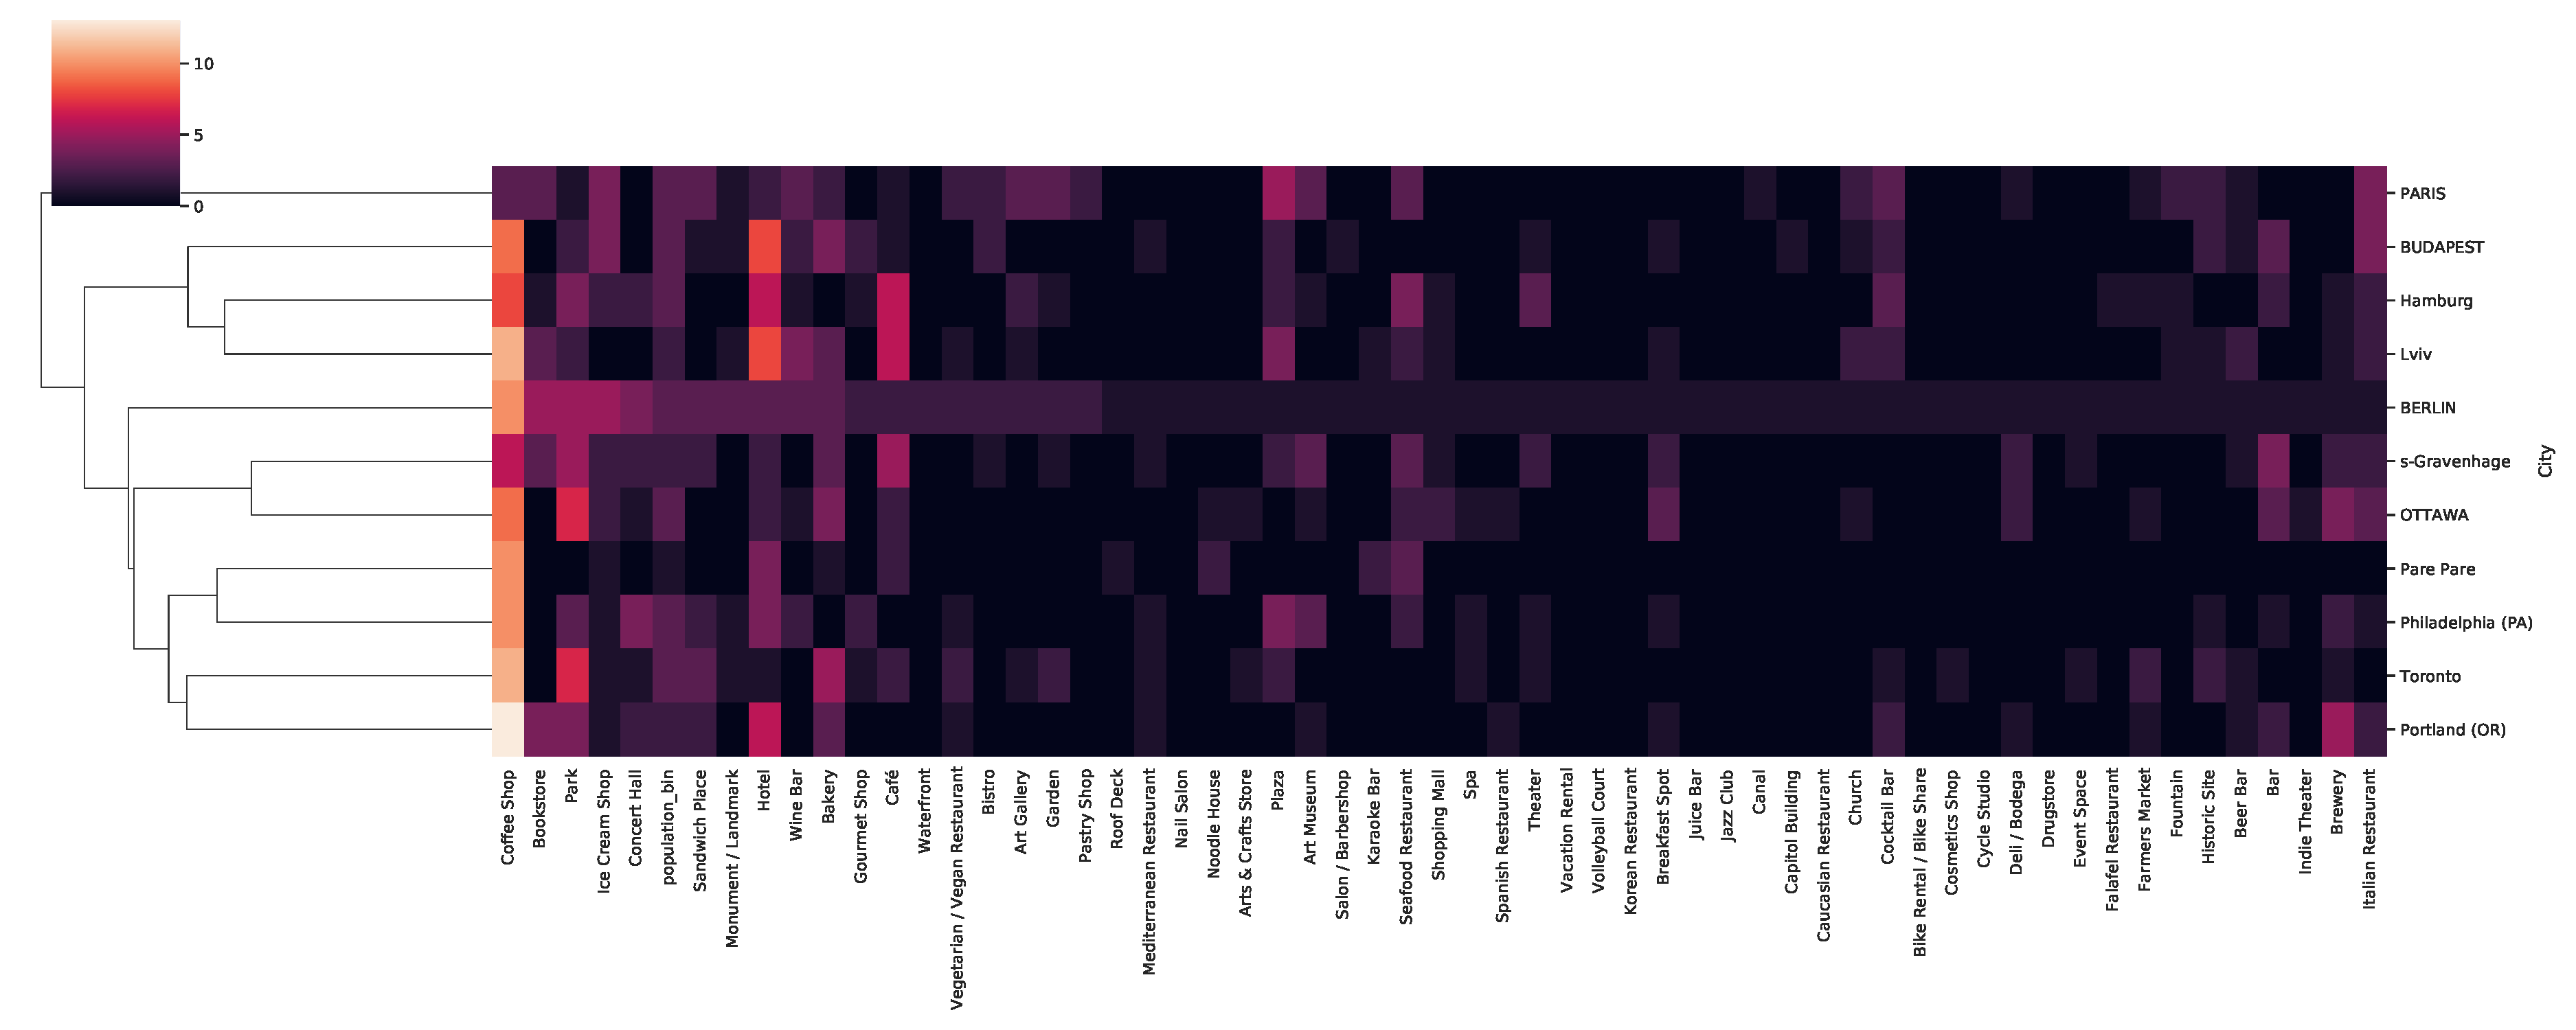
\includegraphics[width = 0.85\textwidth]{figures/heatmap_BERLIN.pdf}
\caption{Heat map representation of the abundance of types of venues per result city. Columns are ordered by abundance in the input city, from most abundant on the left to least abundant on the right. Rows are ordered based on a hierarchical clustering using \texttt{method = 'ward', distance = 'euclidean'}.}\label{fig:heatmap}
\end{center}
\end{figure}

\begin{figure}[h!]
\begin{center}
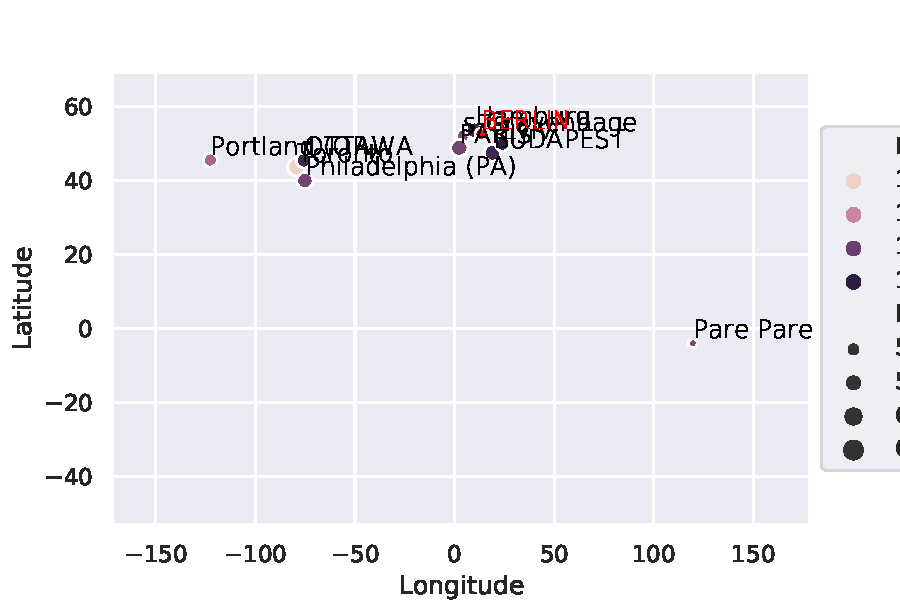
\includegraphics[width = 0.85\textwidth]{figures/worldmap_BERLIN.pdf}
\caption{Scatter plot representation of the cities' coordinates. The input city is highlighted in red while the color of the other cities is a representation of the similarity score. The log10 population size is mapped onto the dot size.}\label{fig:worldmap}
\end{center}
\end{figure}

Because distance can be relevant when choosing the travel destination, \texttt{find\_next\_vacation()} also visualizes the relative location of all result cities in a scatter plot based on longitude and latitude coordinates (see Figure \ref{fig:worldmap}). The color of the dot represent the similarity to the input city (red dot) where the lighter the dot, the more similar this city is to the input city. The size of the dot represents the the population size of the city where the bigger the dot, the more inhabitants this city officially has. Figure \ref{fig:worldmap} reveals two geographical cluster of cities similar to Berlin. There is one European cluster with Hamburg, Paris, and Budapest and one North American cluster with Portland, Toronto, and Philadelphia. The city Pare Pare in Indonesia is a geographical outlier. \\

After carefully considering the results of \texttt{find\_next\_vacation()} I selected s-Gravenhage as for my next vacation because I have never been there, it is close to Berlin, it has a similar cultural landscape to Berlin, while being slightly smaller. To obtain an idea for an itinerary during my vacation I will use the function \texttt{get\_information\_on\_next\_vacation()} to retrieve venues in s-Gravenhage. The result of this call can be found in Table \ref{tab:Gravenhage}. While the data in Figure \ref{fig:heatmap} indicates a wide cultural variety of venues, the results from \texttt{get\_information\_on\_next\_vacation()} indicate only food related venues as top results. 

\begin{table}[h!]
\centering
\scalebox{0.6}{
\begin{tabular}{|l|r|r|l|r|r|l|}
\hline
\textbf{City} & \textbf{City Latitude} & \textbf{City Longitude} & \textbf{Venue} &\textbf{ Venue Latitude} & \textbf{Venue Longitude} & \textbf{Venue Category} \\\hline
s-Gravenhage & 52.07494555 & 4.269680220536451 & De Kaasspeciaalzaak Ed Boele & 52.078563693360294 & 4.269423625840854 & Deli / Bodega \\
s-Gravenhage & 52.07494555 & 4.269680220536451 & cafe madeleine & 52.07875093213555 & 4.276190053614307 & Tea Room \\
s-Gravenhage & 52.07494555 & 4.269680220536451 & Zondag lunchroom & 52.079630346555405 & 4.268465460188677 & Café \\
s-Gravenhage & 52.07494555 & 4.269680220536451 & Restaurant Rakang Thai & 52.0771097635254 & 4.278414389531412 & Thai Restaurant \\
s-Gravenhage & 52.07494555 & 4.269680220536451 & Emma & 52.07672963150343 & 4.282775738593971 & Bar \\
s-Gravenhage & 52.07494555 & 4.269680220536451 & Lokaal Duinoord & 52.08186501187415 & 4.28311407916247 & Bar \\
s-Gravenhage & 52.07494555 & 4.269680220536451 & Spijssalon & 52.07628392465103 & 4.281959093814119 & Ice Cream Shop \\
s-Gravenhage & 52.07494555 & 4.269680220536451 & Indonesisch restaurant Didong & 52.084012194729546 & 4.278235407473984 & Indonesian Restaurant \\
s-Gravenhage & 52.07494555 & 4.269680220536451 & "Koemans Snacks  \&  Broodjes" & 52.078317277178954 & 4.269742793899394 & Snack Place \\\hline
\end{tabular}}\caption{\texttt{get\_information\_on\_next\_vacation('s-Gravenhage', future\_vacation\_destination\_Berlin, 20)}}\label{tab:Gravenhage}
\end{table}

\section{Discussion}
In this report I explored a data set of 2,555 cities. The list of cities with their countries and population size was obtained from the UN website \footnote{\url{https://unstats.un.org/unsd/demographic-social/products/dyb/dyb_2018/}}. The data was not uniformly formatted and I did some manual reformatting. I should also note, that there were some cities missing because their population size was in different columns. If this application was real, one should take good care of creating an extensive list of cities, as the program operates only on the cities given in this original list.\\
For each city, coordinates were obtained using \texttt{geopy}. In general, this worked satisfactory, however sometimes the connection failed. Therefore, I included a column to check whether coordinates had been obtained for a given city in order to restart the loop at the last city that worked. \\
I used the \texttt{Foursquare API} to pull all venues within a 5km radius of each cities coordinates, returning 160,973 venues. Venues were grouped by their venue category as one hot encoding and summarized by city. This lead to the summary of cities with the same name, regardless of their country. This should be improved in a usable version of this application.\\
Exploring the data by reducing the dimensionality of category features into a two dimensional coordinate system showed a dense cloud of cities and a more sparse cluster of outlier cities (see Figure \ref{fig:pca_tsne}). As the color coding indicates, this clustering is not based on population size. Finding an underlying commonality within the outliers should be among future directions for fully exploring the data set.\\
Examining the distribution of venues per city pulled from \texttt{Foursquare} it became evident that \texttt{Foursquare} has a limit of 100 responses per request (see Figure \ref{fig:histograms}). In the future, it would be useful to run the requests multiple times to gather all venues of a city. This would help to make the results of \texttt{find\_next\_vacation()} more accurate.\\
The function \texttt{find\_next\_vacation()} was designed to find the \texttt{k}-most similar cities to a users input city based on the users selected input distance measure. Applying the function to various input cities showed that the function works reliably and returns all desired outputs. The user is provided with the resulting similar cities in a table format, a heat map, and a scatter plot. The table contains all the information, while the heat map visualized the abundance of features and helps the user easily identify the abundance of venue types in each city. The scatter plot helps the user to place the cities based on the geographical location which can be crucial in the decision making process.\\
The function \texttt{get\_information\_on\_next\_vacation()} uses the \texttt{Foursquare API} again to request a selection of venues for a given input city. Currently the input city does not have to be from the resulting table of the previous function.\\
To my regret, I cannot say anything about the validity of these results. It would take more travels to cities selected by the function to find out if the results are reasonable. 


\section{Conclusion}
To conclude, for this Capstone project I developed a method which finds similar cities based on venue data pulled from \texttt{Foursquare} using python libraries such as \texttt{pandas}, \texttt{scipy}, and  \texttt{sklearn}. I demonstrated that I am able to visualize results using special python libraries \texttt{matplotlib} and \texttt{seaborn}. Running through the Ipython notebook I demonstrated, that the methods works in principal but that the results cannot be validated as one would normally do in science.\\
Furthermore, to make this method suitable as a profitable app, I am suggesting these improvements. First, the data set should be more comprehensive, i.e. include more cities and more venues to obtain more accurate results. Second, I would add a broader feature category i.e. grouping Cafes and Coffee shops and having the user select the grouping level for the analysis. Additionally, I would implement an option for feature selection, to accommodate the users preferences, i.e. some might find museums and theaters more important, while others find shopping and nightlife more important.\\
A web-interface such as Flask-App would broaden the methods accessibility also to non-coders. In this app one should only need to input a city and the feature selection. The app automatically creates the one-hot encoding and runs \texttt{find\_next\_vacation()}, returning the resulting cities as table, and visualizing the results in a heat map and scatter plot. Based on the result table, the user can then click on a city and get all the venues in this city.\\
With these improvements, I believe, that my method poses a great app for travelers of all kinds.

\end{document}